\documentclass{article}                                                         
\usepackage[french]{babel}
\usepackage{geometry}
\geometry{hmargin=2.5cm,vmargin=1.5cm} 
\usepackage[T1]{fontenc}
\usepackage{tcolorbox,listings}
\usepackage{fullpage}
\usepackage{color}
\usepackage{graphicx}
\usepackage{float}
\usepackage[utf8]{inputenc}                                                    
\usepackage{algorithmeUTF8}
\usepackage{verbatim}
\lstset{
language=C,
literate=
{²}{{\textsuperscript{2}}}1
{⁴}{{\textsuperscript{4}}}1
{⁶}{{\textsuperscript{6}}}1
{⁸}{{\textsuperscript{8}}}1
{€}{{\euro{}}}1
{’}{'}1
{○}{{$ \circ $}}1
{●}{{$ \bullet $}}1
{é}{{\'e}}1
{è}{{\`{e}}}1
{ê}{{\^{e}}}1
{ë}{{\¨{e}}}1
{É}{{\'{E}}}1
{Ê}{{\^{E}}}1
{û}{{\^{u}}}1
{ù}{{\`{u}}}1
{â}{{\^{a}}}1
{à}{{\`{a}}}1
{á}{{\'{a}}}1
{ã}{{\~{a}}}1
{Á}{{\'{A}}}1
{Â}{{\^{A}}}1
{Ã}{{\~{A}}}1
{ç}{{\c{c}}}1
{Ç}{{\c{C}}}1
{õ}{{\~{o}}}1
{ó}{{\'{o}}}1
{ô}{{\^{o}}}1
{Õ}{{\~{O}}}1
{Ó}{{\'{O}}}1
{Ô}{{\^{O}}}1
{î}{{\^{i}}}1
{Î}{{\^{I}}}1
{í}{{\'{i}}}1
{Í}{{\~{Í}}}1,  
basicstyle=\ttfamily,
stringstyle=\ttfamily\color{green!50!black},
keywordstyle=\color{blue}\bfseries,
commentstyle=\color{red!50!black}\itshape,
showspaces=false,
showstringspaces=true,
fontadjust=true,
keepspaces=true,
flexiblecolumns=true,
frame=single,
upquote=true
}


\lstdefinestyle{frameStyle}{
basicstyle=\footnotesize,
numbers=left,
numbersep=20pt,
numberstyle=\tiny\color{black}
}

\tcbuselibrary{listings,skins,breakable}

\newtcblisting{customFrame}{
arc=0mm,
top=0mm,
bottom=0mm,
left=3mm,
right=0mm,
width=\textwidth,
listing only,
listing options={style=frameStyle},
breakable
}

\title{RAPPORT PROJET OTHELLO}                         
\author{Victorin Turnel, Paul Thulliez,Chen Yang, Ahmed Zarki, Sacha Wojciechowski}

\begin{document}
\maketitle
\tableofcontents

\section{Introduction}
Le jeu d'Othello, également connu sous le nom de Reversi, est un jeu de stratégie abstraite qui a été inventé au milieu du XIXe siècle. Bien que les règles du jeu soient simples, les possibilités de jeu sont infinies, ce qui en fait un défi stimulant pour les joueurs de tous niveaux.


C'est ainsi que dans le cadre du cours d'Algorithmique avancée, nous avons eu à réaliser le développement d'un jeu d'Othello. Nous détaillerons dans ce rapport les différentes étapes qui nous ont permis de parvenir à ce résultat. Pour cela, ce document détaillera chaque étape du cycle en V dans l'ordre. 


Pour continuer, nous allons détailler les principaux objectifs de ce projet. Le but de ce projet était le développement d'un jeu d'Othello ayant plusieurs fonctionnalités :
\begin{itemize}
    \item Un programme de base permettant de jouer à l'Othello
    \item Une interface Homme-Machine fonctionnelle
    \item Une intelligence artificielle
    \item Un programme permettant l'intégration d'un mode tournois
    \item Une interface Machine-Machine
    \item Une documentation
    \item Des tests unitaires
\end{itemize}

Enfin, rappelons les règles de l'Othello. Le jeu se joue sur un plateau de huit rangées et huit colonnes, avec deux joueurs qui s'affrontent. Les joueurs ont chacun des pions de couleur, généralement noirs et blancs. Le but du jeu est de finir avec le plus de pions de sa couleur sur le plateau.

Le joueur qui commence le jeu place son pion au centre du plateau, et les joueurs jouent à tour de rôle. À chaque tour, un joueur doit placer son pion sur le plateau de manière à ce qu'il encercle au moins un pion adverse, formant ainsi une chaîne de pions de sa couleur. Les pions encerclés sont alors retournés pour prendre la couleur du joueur qui vient de jouer. Si un joueur ne peut pas jouer, il doit passer son tour.

Le jeu se termine lorsque tous les emplacements du plateau sont occupés ou lorsque aucun joueur ne peut plus jouer. Le joueur qui a le plus de pions de sa couleur sur le plateau à la fin du jeu est déclaré vainqueur. Si le nombre de pions de chaque couleur est égal, la partie est déclarée nulle.

\section{Analyse}

\subsection{TAD COULEUR :}
\begin{tad}
\tadNom{Couleur}
\tadDependances{Booleen}

\begin{tadOperations}{couleur}  
\tadOperation{blanc}{\tadUnParam{Couleur}}
\tadOperation{noir}{\tadUnParam{Couleur}}
\tadOperation{estBlanc}{\tadUnParam{Couleur}}{\tadUnParam{Booleen}}
\tadOperation{changerCouleur}{\tadUnParam{Couleur}}{\tadUnParam{Couleur}}
\end{tadOperations}

\begin{tadAxiomes}
\tadAxiome{estBlanc(blanc())}
\tadAxiome{non(estBlanc(noir()))}
\tadAxiome{changerCouleur(blanc())=noir()}
\end{tadAxiomes}

\end{tad}

\subsection{TAD PION :}
\begin{tad}
\tadNom{Pion}
\tadDependances{Couleur}

\begin{tadOperations}{creerPion}  
\tadOperation{creerPion}{\tadUnParam{Couleur}}{\tadUnParam{Pion}}
\tadOperation{obtenirCouleurSuperieure}{\tadUnParam{Pion}}{\tadUnParam{Couleur}}
\tadOperation{retournerPion}{\tadUnParam{Pion}}{\tadUnParam{Pion}}
\end{tadOperations}

\begin{tadAxiomes}
\tadAxiome{obtenirCouleurSuperieure(retournerPion(creerPion(col) != col}
\end{tadAxiomes}

\end{tad}


\subsection{TAD POSITION :}
\begin{tad}
	\tadNom{Position}
	\tadDependances{1..8}
	\begin{tadOperations}{Position}
		\tadOperation{position}{\tadDeuxParams{1..8}{1..8}}{Position}
		\tadOperation{obtenirX}{Position}{1..8}
		\tadOperation{obtenirY}{Position}{1..8}
	\end{tadOperations}
	\begin{tadAxiomes}
		\tadAxiome{obtenirX(Position(x,y))=x}
		\tadAxiome{obtenirY(Position(x,y))=y}
	\end{tadAxiomes}
	
	
\end{tad}


\subsection{TAD COUP :}
\begin{tad}
	\tadNom{Coup}
	\tadDependances{Pion,Pion,Position}
	\begin{tadOperations}{Coup}
		\tadOperation{coup}{Pion,Position}{\tadUnParam{Coup}}
		\tadOperationAvecPreconditions{obtenirPionCoup}{Coup}{Pion}
		\tadOperationAvecPreconditions{obtenirPositionCoup}{\tadUnParam{Coup}}{Position}
        \end{tadOperations}
              
	\begin{tadAxiomes}
          \tadAxiome{obtenirPionCoup(coup(pion,pos))=pion}
          \tadAxiome{obtenirPositionCoup(coup(pion,pos))=pos}
	\end{tadAxiomes}


\end{tad}

\subsection{TAD COUPS :}
\begin{tad}
	\tadNom{Coups}
	\tadDependances{Coup, NNN, Naturel}
	\begin{tadOperations}{Coups}
		\tadOperation{coups}{}{\tadUnParam{Coups}}
		\tadOperation{nbCoups}{Coups}{Naturel}
		\tadOperation{ajouterCoups}{\tadDeuxParams{Coups}{Coup}}{Coups}
		\tadOperationAvecPreconditions{iemeCoup}{\tadDeuxParams{Coups}{NNN}}{Coup}
	\end{tadOperations}
	\begin{tadPreconditions}{Coups}
		\tadPrecondition{iemeCoups(coups,position)}{position $\leq$ nbCoups(coups)}
	\end{tadPreconditions}
	\begin{tadAxiomes}
		\tadAxiome{nbCoups(Coups())=0}
		\tadAxiome{nbCoups(ajouterCoups(coups,coup)) = nbCoups(coups) +1}
		\tadAxiome{iemeCoup(ajouterCoups(coups,coup),nbCoups(coups)+1 ) = coup}
	\end{tadAxiomes}


\end{tad}
        


\subsection{TAD PLATEAU :}

\begin{tad}


\tadNom{Plateau}
\tadDependances{Pion, Position, \booleen}

\begin{tadOperations}{retournerPion}
	\tadOperation{plateau}{}{\tadUnParam{Plateau}}
	\tadOperationAvecPreconditions{poserPion}{\tadTroisParams{Plateau}{Position}{Pion}}{\tadUnParam{Plateau}}
	\tadOperationAvecPreconditions{obtenirPion}{\tadDeuxParams{Plateau}{Position}}{\tadUnParam{Pion}}
	\tadOperation{estCaseVide}{\tadDeuxParams{Plateau}{Position}}{\tadUnParam{\booleen}}
	\tadOperationAvecPreconditions{retournerPion}{\tadDeuxParams{Plateau}{Position}}{\tadUnParam{Plateau}}
	\tadOperationAvecPreconditions{enleverPion}{\tadDeuxParams{Plateau}{Position}}{\tadUnParam{Plateau}}
\end{tadOperations}

\begin{tadPreconditions}{poserPion(pos,pion,pl)}
	\tadPrecondition{obtenirPion(pos,pl)}{non (estCaseVide(pos,pl))}	
	\tadPrecondition{retournerPion(pos,pl)}{non (estCaseVide(pos,pl))}
	\tadPrecondition{poserPion(pos,pion,pl)}{estCaseVide(pos,pl)}
	\tadPrecondition{enleverPion(pos,pl)}{non (estCaseVide(pos,pl))}
\end{tadPreconditions}

\begin{tadAxiomes}
	\tadAxiome{estCaseVide(pos,plateau())}
	\tadAxiome{obtenirPion(pos,poserPion(pos,pion,plateau()))= pion}
	\tadAxiome{estCaseVide(pos,enleverPion(pos,plateau()))}
	\tadAxiome{non estCaseVide(pos,poserPion(pos,pion,plateau()))}
	\tadAxiome{retournerPion(pos,retournerPion(pos,pl))=pl}	
\end{tadAxiomes}
\end{tad}



\subsection{Analyse descendante de la fonction faireUnePartie}

\begin{figure}[H]
    \rotatebox{90}{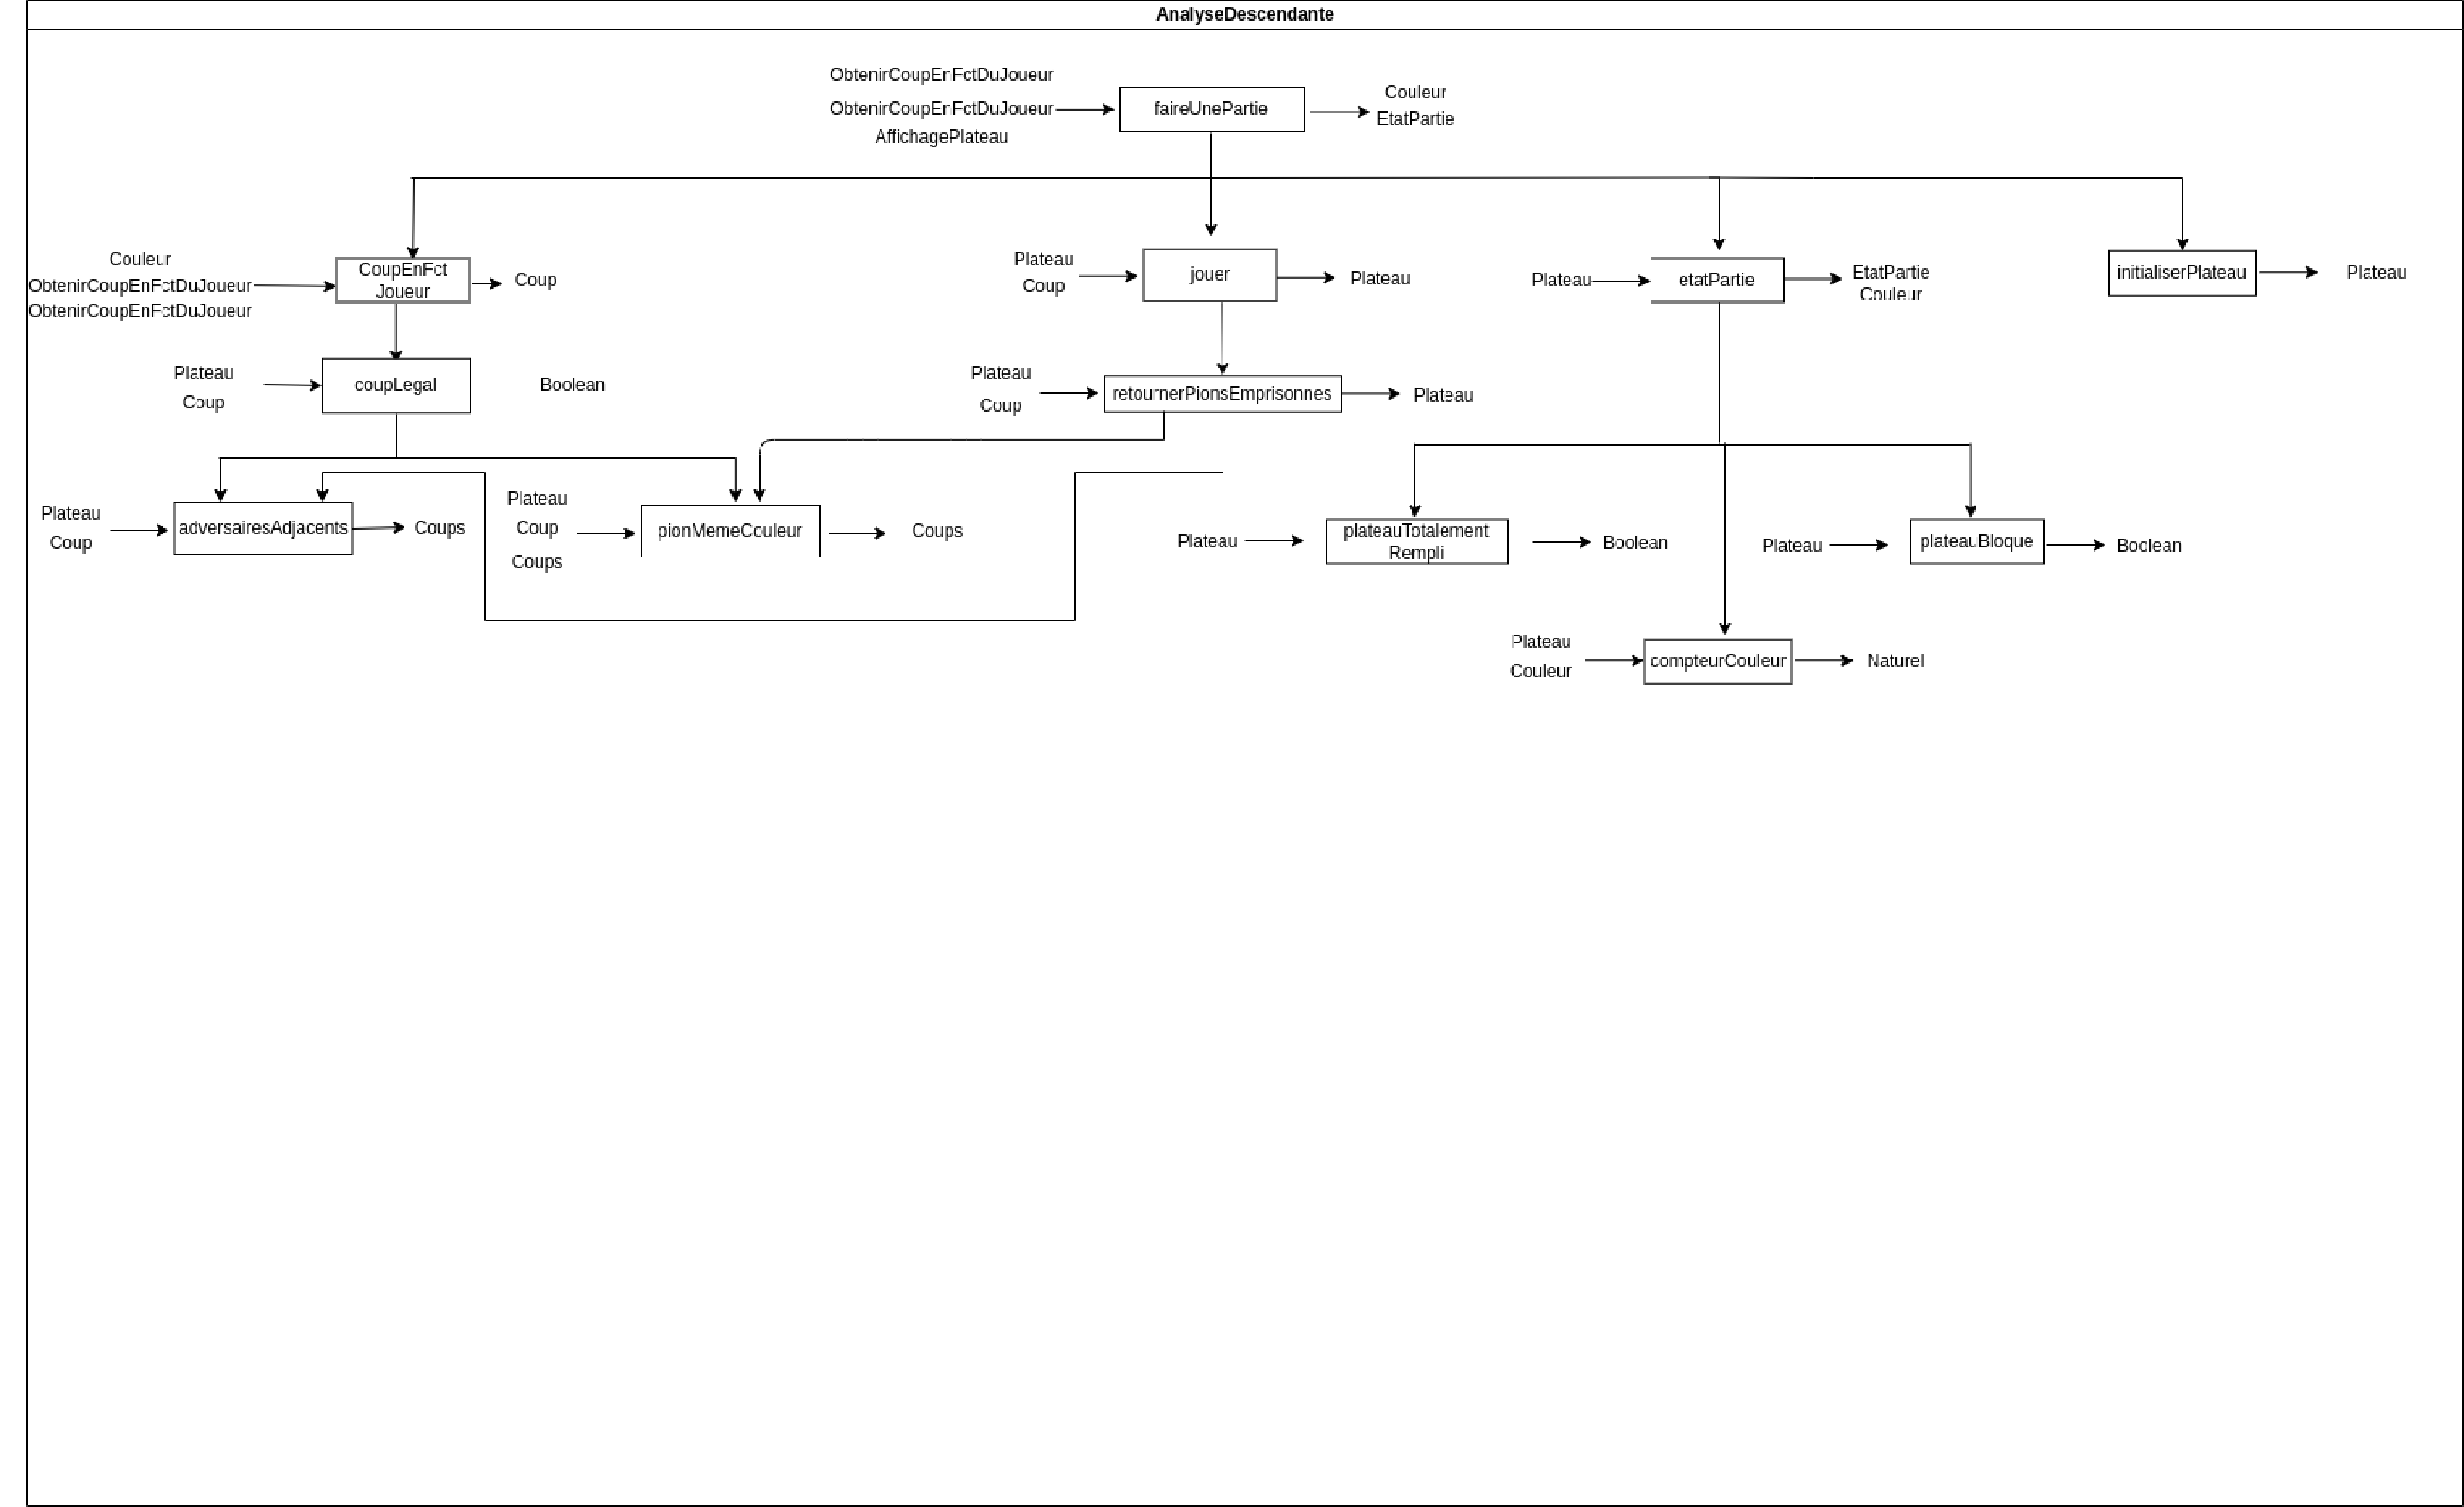
\includegraphics[width=23cm,height=15cm]{analyse/ADFaireUnePartieV6.pdf}}
    \caption{Analyse descendante de faireUnePartie}
    \label{un-identifiant1}
\end{figure}

\subsection{Analyse descendante de la fonction obtenirCoup}

\begin{figure}[H]                                                                                                                                                                                             
    \rotatebox{90}{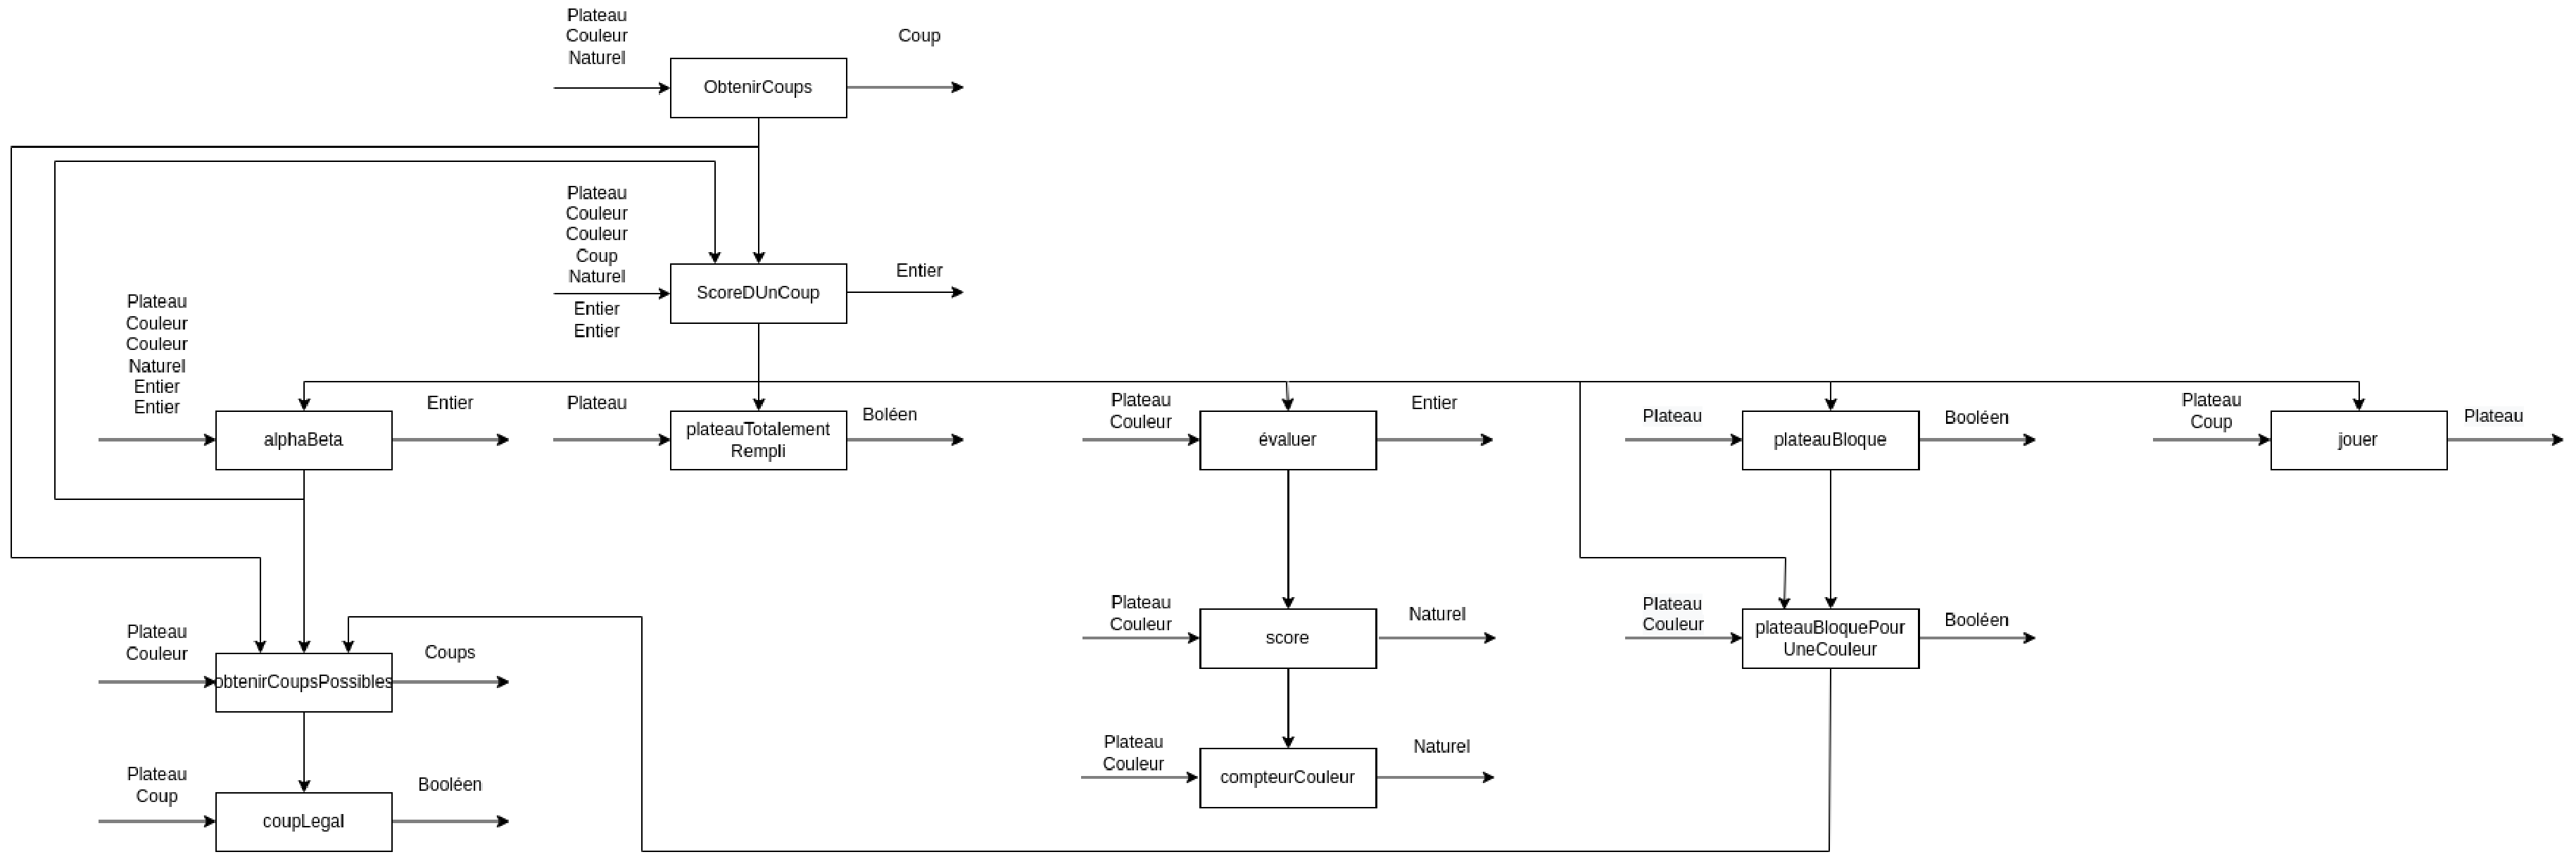
\includegraphics[width=23cm,height=10cm]{analyse/ADobtenirCoup.pdf}}                                                                                                               
    \caption{Analyse descendante de obtenirCoup}                                                                                                                          
    \label{un-identifiant2}                                                                                                                                                                                 
\end{figure}       

\section{Conception préliminaire}

\subsection{TAD : Couleur}
\begin{algorithme}
	\signaturefonction{couleurBlanc}{}{Couleur}
	\signaturefonction{couleurNoir}{}{Couleur}
	\signaturefonction{couleurEstBlanc}{c : Couleur}{\booleen}
  	\signaturefonction{couleurChangerCouleur}{couleur:Couleur}{Couleur}
\end{algorithme}


\subsection{TAD : Pion}
\begin{algorithme}
  \signaturefonction{creerPion}{couleur : Couleur}{Pion}
  \signaturefonction{obtenirCouleurSuperieure}{pion : Pion}{Couleur}
  \signatureprocedure{retournerPion}{\paramEntree{pion : Pion},\paramSortie{Pion}}
\end{algorithme}
  


\subsection{TAD : Position}
\begin{algorithme}
	\signaturefonction
	{position}
	{largeur : \textbf{1..8}, hauteur : \textbf{1..8}}
	{\textbf{Position}}
	
	\vspace*{5mm}
	
	\signaturefonction
	{obtenirX}
	{unePosition : \textbf{Position}}
	{\textbf{1..8}}
	
	\vspace*{5mm}
	
	\signaturefonction
	{obtenirY}
	{unePosition : \textbf{Position}}
	{\textbf{1..8}}
	
	
	
\end{algorithme}




\subsection{TAD : Coup}
\begin{algorithme}
\signaturefonction{coupCoup}{pion:Pion}{Coup}
\signaturefonction{coupObtenirPionCoup}{coup:Coup}{Pion}
\signaturefonction{coupObtenirPositionCoup}{coup:Coup}{Position}
\end{algorithme}


\subsection{TAD : Plateau}
\begin{algorithme}
  \signaturefonction{plateau}{}{Plateau}
  \signatureprocedure{poserPion}{\paramEntreeSortie{plateau : Plateau} , \paramEntree{pos : Position , pion: Pion}}

  \vspace*{5mm}
  
  \preconditions{estCaseVide(plateau , pos)}

  \vspace*{5mm}
  
  \signaturefonction{obtenirPion}{plateau : Plateau , pos : Position}{Pion}

  \vspace*{5mm}

  \preconditions{non (estCaseVide(plateau , pos)}

  \vspace*{5mm}
  
  \signaturefonction{estCaseVide}{plateau : Plateau , pos : Position}{\booleen}

  \vspace*{5mm}
  
  \signatureprocedure{retournerPion}{\paramEntreeSortie{plateau : Plateau} , \paramEntree{pos : Position}}

  \vspace*{5mm}
  
  \preconditions{non (estCaseVide(plateau , pos)}

  \vspace*{5mm}
  
  \signatureprocedure{enleverPion}{\paramEntreeSortie{plateau : Plateau},\paramEntree{pos : Position}}

  \vspace*{5mm}
  
  \preconditions{non (estCaseVide(plateau , pos)}
\end{algorithme}


\subsection{faireUnePartie}
\begin{algorithme}
  \type{EtatPartie}{[TERMINE,ENCOURS,EGALITE]}
\end{algorithme}

\vspace*{5mm}

\begin{algorithme}
  \type{Sortie}{\signatureprocedure{}{\paramEntree{plateau : \textbf{Plateau}, coup : \textbf{Coup}, possibilite : \booleen}}}
\end{algorithme}

\vspace*{5mm}

\begin{algorithme}
  \type{ObtenirCoupEnFctDuJoueur}{\signaturefonction{}{plateau : \textbf{Plateau}, joueur : \textbf{Couleur}, profondeur:\naturel}}{\textbf{Coup}}
\end{algorithme}

\vspace*{5mm}

\begin{algorithme}
  \signatureprocedure{faireUnePartie}{\paramEntree{obtenirCoupBlanc,obtenirCoupJoueurNoir : \textbf{ObtenirCoupEnFctDuJoueur}, sortie : \textbf{Sortie}} \paramSortie{couleurGagnant : \textbf{Couleur}, etat : \textbf{EtatPartie}}}
  
  \vspace*{5mm}
  
  \signaturefonction{initialiserPlateau}{}{\textbf{Plateau}}

  \vspace*{5mm}
  
  \signatureprocedure{etatPartie}{\paramEntree{plateau : \textbf{Plateau}}, \paramSortie{couleur: \textbf{Couleur}, etat: \textbf{EtatPartie}}}

  \vspace*{5mm}
  
  \signaturefonction{compteurCouleur}{plateau : \textbf{Plateau}, couleur : \textbf{Couleur}}{\naturel}

  \vspace*{5mm}
  
  \signaturefonction{plateauBloque}{plateau : \textbf{Plateau}}{\booleen}

  \vspace*{5mm}
  
  \signatureprocedure{jouer}{\paramEntreeSortie {plateau : \textbf{Plateau}} , \paramEntree{coup : \textbf{Coup}}}
  
  \vspace*{5mm}
  
  \signaturefonction{coupLegal}{plateau : \textbf{Plateau} , coup : \textbf{Coup}}{\booleen}

  \vspace*{5mm}
  \signatureprocedure{retournerPionsEmprisonnes}{\paramEntreeSortie{plateau : \textbf{Plateau}} , \paramEntree{coup : \textbf{Coup}}}

  \vspace*{5mm}
  
  \signaturefonction{adversairesAdjacents}{plateau : \textbf{Plateau} , coup : \textbf{Coup}}{\textbf{Coups}}

  \vspace*{5mm}
  
  \signaturefonction{pionMemeCouleur}{plateau : \textbf{Plateau} , coup : \textbf{Coup}, pionsLegals : \textbf{Coups}}{\textbf{Coups}}

  \vspace*{5mm}
  
  \signaturefonction{coupEnFctJoueur}{obtenirCoupBlanc,obtenirCoupNoir : \textbf{ObtenirCoupEnFctDuJoueur}, couleur : \textbf{Couleur}, plateau : \textbf{Plateau}}{\textbf{Coup}}
\end{algorithme}



\subsection{obtenirCoup}
\documentclass{article}
\usepackage{algorithmeUTF8}
\begin{document}
	\begin{algorithme}
		\signaturefonction
		{obtenirCoup}
		{unPlateau : \textbf{Plateau}, joueur : \textbf{Couleur}, profondeur : \naturel}
		{\textbf{Coup}}
		\preconditions{non plateauComplet(unPlateau)}
		
		\vspace{5mm}
		
		
		\signaturefonction
		{scoreDUnCoup}
		{unPlateau : \textbf{Plateau}, joueurRef, joueurCourant : \textbf{Couleur}, unCoup : \textbf{Coup}, profondeur : \naturel, alpha, beta : \entier}
		{\entier}
		
		\vspace{5mm}
		
		
		\signaturefonction
		{alphaBeta}
		{unPlateau : \textbf{Plateau}, joueurRef, joueurCourant : \textbf{Couleur}, profondeur : \naturel, alpha, beta : \entier}
		{\entier}
		
		\vspace{5mm}
		
		
		\signaturefonction
		{plateauTotalmentRempli}
		{unPlateau : \textbf{Plateau}}
		{\booleen}
		
		\vspace{5mm}
		
		
		\signaturefonction
		{evaluer}
		{unPlateau : \textbf{Plateau}, joueurRef : \textbf{Couleur}}
		{\entier}
		
		\vspace{5mm}
		
		
		\signaturefonction
		{score}
		{unPlateau : \textbf{Plateau}, joueur : \textbf{Couleur}}
		{\naturel}
		
		\vspace{5mm}
		
		
		\signaturefonction
		{obtenirCoupsPossibles}
		{unPlateau : \textbf{Plateau}, joueurRef : \textbf{Couleur}}
		{\textbf{Coups}}
		
		\vspace{5mm}
		
		\signaturefonction
		{compteurCouleur}
		{plateau : \textbf{Plateau}, couleur : \textbf{Couleur}}
		{\naturel}
		
		\vspace{5mm}
		
		\signaturefonction
		{compteurCouleur}
		{plateau : \textbf{Plateau}, couleur : \textbf{Couleur}}
		{\naturel}
		
		\vspace{5mm}
		
		\signaturefonction
		{plateauBloquePourUneCouleur}
		{unPlateau : \textbf{Plateau}, laCouleur : \textbf{Couleur}}
		{\booleen}
		
		\vspace{5mm}
		
		\signaturefonction
		{plateauBloque}
		{unPlateau : \textbf{Plateau}}
		{\booleen}
		
		\vspace{5mm}
		
		\signaturefonction
		{coupLegal}
		{unPlateau : \textbf{Plateau}, unCoup : \textbf{Coup}}
		{\booleen}
		
	\end{algorithme}
\end{document}




\section{Conception détaillée}
\subsection{Conception détaillée des fonctions des TAD :}

\subsubsection{TAD COULEUR :}
\begin{algorithme}
  \type{Couleur}{\{Blanc,Noir\}}
\end{algorithme}

  \vspace*{5mm}


\begin{algorithme}
  \small
  \fonction{blanc}{}{Couleur}
  {}
    {\retourner{Blanc}}

\end{algorithme}


  \vspace*{5mm}

\begin{algorithme}
  \small
  \fonction{noir}{}{Couleur}
  {}
   {\retourner{Noir}}

\end{algorithme}

  \vspace*{5mm}

\begin{algorithme}
  \small
  \fonction{estBlanc}{couleur:Couleur}{\booleen}
  {}
  {\retourner{couleur=Blanc}}

\end{algorithme}

  \vspace*{5mm}

\begin{algorithme}
  \small
  \fonction{changerCouleur}{couleur:Couleur}{Couleur}
  {}
  {\sialorssinon{estBlanc(couleur)}{\affecter{couleur}{Noir} \retourner{couleur}}{\affecter{couleur}{Blanc} \retourner{couleur}}}

\end{algorithme}


\subsubsection{TAD PION :}
\begin{algorithme}
  \begin{enregistrement}{\textbf{Pion}}
    \champEnregistrement{couleur : \textbf{Couleur}}
  \end{enregistrement}
\end{algorithme}

\vspace*{5mm} 

\begin{algorithme}
  \small
  \fonction
      {creerPion}
      {couleur : \textbf{Couleur}}
      {\textbf{Pion}}
      {pion : \textbf{Pion}}
      {{\affecter{pion.Couleur}{couleur}}

        {\retourner {pion}}}
\end{algorithme}

\vspace*{5mm} 

\begin{algorithme}
  \small
  \fonction
      {obtenirCouleurSuperieure}
      {pion : \textbf{Pion}}
      {\textbf{Couleur}}
      {couleur : \textbf{Couleur}}
      {\retourner {pion.Couleur}}
\end{algorithme}

\vspace*{5mm} 

\begin{algorithme}
  \small
  \procedure
      {retournerPion}
      {\paramEntreeSortie{pion : \textbf{Pion}}}
      {}
      {\instruction{changeCouleur(pion.Couleur)}}
\end{algorithme}


\subsubsection{TAD POSITION :}
\begin{algorithme}
	
	\begin{enregistrement}{Pion}
		\champEnregistrement{x}{\textbf{1..LARGEUR\_PLATEAU}}
		\champEnregistrement{y}{\textbf{1..HAUTEUR\_PLATEAU}}
	\end{enregistrement}
	
	\vspace*{5mm} 
	
	\fonction
	{position}
	{largeur : \textbf{1..LARGEUR\_PLATEAU}, hauteur : \textbf{1..HAUTEUR\_PLATEAU}}
	{\textbf{Position}}
	{resultat : Position}
	{\affecter{resultat.x}{largeur}
		\affecter{resultat.y}{hauteur}
		\retourner {resultat}}
	
	\vspace*{5mm} 
	
	\fonction
	{obtenirX}
	{unePosition : \textbf{Position}}
	{\textbf{1..LARGEUR\_PLATEAU}}
	{}
	{\retourner {pion.x}}
	
	\vspace*{5mm} 
	
	\fonction
	{obtenirY}
	{unePosition : \textbf{Position}}
	{\textbf{1..HAUTEUR\_PLATEAU}}
	{}
	{\retourner {pion.y}}
	
	
\end{algorithme}

\subsubsection{TAD COUP :}
\begin{algorithme}
  \begin{enregistrement}{\textbf{Coup}}
    \champEnregistrement{pion}{\textbf{Pion}}
    \champEnregistrement{position}{\textbf{Position}}
  \end{enregistrement}
\end{algorithme}

\vspace*{5mm}

\begin{algorithme}
  \small
  \fonction
      {coupCoup}
      {pion :\textbf{Pion}, pos : \textbf{Position}}
      {\textbf{Coup}}
      {}
      {
        \affecter{coup.position}{pos}
        \affecter{coup.pion}{pion}
        \retourner{coup}
      }
      
\end{algorithme}

\vspace*{5mm}

\begin{algorithme}
  \small
  \fonction
      {coupObtenirPionCoup}
      {coup : \textbf{Coup}}
      {\textbf{Pion}}
      {}
      {
        \retourner{coup.pion} 
      }
      
\end{algorithme}

\vspace*{5mm}

\begin{algorithme}
  \small
  \fonction
      {coupObtenirPositionCoup}
      {coup : \textbf{Coup}}
      {\textbf{Position}}
      {}
      {
        \retourner{coup.position}
      }
      
\end{algorithme}


\subsubsection{TAD COUPS :}
\begin{algorithme}
	
	\begin{enregistrement}{Coups}
		\champEnregistrement{lesCoups}{\textbf{Tableau[1..LARGEUR\_PLATEAU*HAUTEUR\_PLATEAU] de Coup}}
		\champEnregistrement{nbTotalCoups}{\naturel}
	\end{enregistrement}
	
	\vspace*{5mm} 
	
	\fonction
	{coups}
	{}
	{\textbf{Coups}}
	{resultat : Coups}
	{\affecter{resultat.nbTotalCoups}{0}
		\retourner {resultat}}
	
	\vspace*{5mm} 
	
	\fonction
	{nbCoups}
	{cps : \textbf{Coups}}
	{\naturel}
	{}
	{\retourner {cps.nbTotalCoups}}
	
	\vspace*{5mm} 
	
	\procedure
	{ajouterCoups}
	{\paramEntreeSortie{cps : \textbf{Coups}},\paramEntree{unCoup : \textbf{Coup}}}
	{}
	{\affecter{cps.nbTotalCoups}{cps.nbTotalCoups+1}
		\affecter{cps.lesCoups[cps.nbTotalCoups]}{unCoup}}
	
	\vspace*{5mm} 
	
	\fonction
	{iemeCoup}
	{cps : \textbf{Coups}, place : \textbf{NNN} }
	{\textbf{Coup}
		\preconditions{place $\leq$ nbCoups(coups)}}
	{}
	{\retourner {cps.lesCoups[place]}}
	
	
\end{algorithme}

\subsubsection{TAD PLATEAU :}

\begin{algorithme}
	\begin{enregistrement}{Case}
		\champEnregistrement{estVide}{\booleen}
		\champEnregistrement{pion}{Pion}
	\end{enregistrement}
	\vspace*{5mm}
\end{algorithme}
\begin{algorithme}
	\type{Plateau}{Tableau[8][8] de \textbf{Case}}
\end{algorithme}
	\vspace*{5mm}
		
\begin{algorithme}
	\fonction {plateau}{}{Plateau}{plateau : \textbf{Plateau} , i,j:\naturel}{
	\pour{i}{1}{8}{}
		{\pour{j}{1}{8}{}
		{\affecter{plateau[i][j].estVide}{Vrai}}
		}
	\retourner {plateau}
	}
	\vspace*{5mm}	
	\fonction{initialiser}{}{Plateau}{plateau : Plateau , pion : Pion , blanc : Couleur}{
	\affecter{plateau}{plateau()}
	\affecter{blanc}{couleurBlanc()}
	\affecter{pion}{creerPion(blanc)}       
    	\instruction{poserPion(plateau,position(4,4),pion)}
    	\instruction{poserPion(plateau,position(5,5),pion)}
    	\instruction{Pion.retournerPion(pion)}
    	\instruction{poserPion(plateau,position(4,5),pion)}
    	\instruction{poserPion(plateau,position(5,4),pion)}
    	\retourner{p}
    	}
    	\vspace*{5mm}
    	\procedureAvecPreconditions{poserPion}
    	{\paramEntreeSortie {plateau : Plateau} , \paramEntree {pos : Position , pion : Pion}}
    	{estCaseVide(pos,plateau)}
    	{x,y : \textbf{1...8}}
    	{\affecter{x}{obtenirX(pos)}
    	\affecter{y}{obtenirY(pos)}
    	\affecter{plateau[x][y].pion}{pion}
    	\affecter{plateau[x][y].estVide}{Faux}}
    	\vspace*{5mm}
    	\fonctionAvecPreconditions{obtenirPion}
    	{pos : Position , plateau : Plateau}
    	{Pion}
    	{non estCaseVide(plateau,pos)}
    	{x,y : \textbf{1...8}}
    	{\affecter{x}{obtenirX(pos)}
    	\affecter{y}{obtenirY(pos)}
    	\retourner {plateau[x][y].pion}
    	}
    	\vspace*{5mm}
    	\procedureAvecPreconditions{retournerPion}
    	{\paramEntreeSortie {plateau : Plateau} , \paramEntree{pos : Position}}
    	{non estCaseVide(plateau,pos)}
    	{pion : Pion}
    	{
    	\affecter{pion}{obtenirPion(pos , plateau)}
    	\instruction{Pion.retournerPion(pion)}
    	\instruction{enleverPion(plateau,pos)}
    	\instruction{poserPion(plateau,pos,pion)}
  	}
  	\vspace*{5mm}
  	\fonction{estCaseVide}{plateau : Plateau , pos : Position}{\booleen}
  	{x,y : \textbf{1...8}}
  	{\affecter{x}{obtenirX(pos)}
    	\affecter{y}{obtenirY(pos)}
    	\retourner {plateau[x][y].estVide}
    	}
    	\vspace*{5mm}
    	\procedureAvecPreconditions{enleverPion}
    	{\paramEntreeSortie{plateau : Plateau} , \paramEntree{pos : Position}}
    	{non estCaseVide(plateau,pos)}
    	{x,y : \textbf{1...8}}
    	{\affecter{x}{obtenirX(pos)
    	\affecter{y}{obtenirY(pos)}
    	\affecter{plateau[x][y].estVide}{Vrai}}
    	}
     
\end{algorithme}



\subsection{Conception détaillée des fonctions d'obtenirCoup}
\begin{algorithme}
	\small
	\fonction
	{obtenirCoup}
	{unPlateau : \textbf{Plateau}, joueur : \textbf{Pion}, profondeur : \naturel}
	{\textbf{Coup}}
	{resultat : \textbf{Coup}, cps : \textbf{Coups}, score, meilleurScore : \entier, i : \naturel}
	{\affecter{cps}{obtenirCoupsPossibles(unPlateau)}
		\affecter{resultat}{ieme(cps,1)}
		\affecter{meilleurScore}{scoreDUnCoup(unPlateau,resultat,joueur,joueur,profondeur)}
		\pour{i}{2}{nb(cps)}{}
		{
			\affecter{score}{scoreDUnCoup(unPlateau,ieme(cps,i),joueur,joueur,profondeur)}
			\sialors{score $>$ meilleurScore}
			{
				\affecter{resultat}{ieme(cps,i)}
				\affecter{meilleurScore}{score}
			}
		}
		\retourner{resultat}
	}
	
	\vspace*{1cm}
	
	\small
	\fonction
	{obtenirCoupsPossibles}
	{unPlateau : \textbf{Plateau}, joueurRef : \textbf{Pion}}
	{\textbf{Coups}}
	{resultat : \textbf{Coups}, i : \naturel, temp : \textbf{Position}}
	{	\affecter{resultat}{coups()}
		\pour{i}{1}{HAUTEUR\_PLATEAU}{}
		{
			\pour{j}{1}{LARGEUR\_PLATEAU}{}
			{
				\affecter{coupTemp}{coup(joueurRef,position(j,i))}
				\sialors{coupLegal(unPlateau,coupTemp)}
				{
					\instruction{ajouterCoups(resultat,temp)}
				}
			}
			
		}
		\retourner{resultat}
	}
	
	\vspace*{1cm}
	
	\small
	\fonction
	{evaluer}
	{unPlateau : \textbf{Plateau}, joueurRef : \textbf{Pion}}
	{\entier}
	{}
	{	\retourner{\instruction{score(unPlateau,joueurRef)-score(unPlateau,joueurRef)}}
	}
	
	\vspace*{1cm}
	
	\small
	\fonction
	{scoreDUnCoup}
	{unPlateau : \textbf{Plateau}, joueurRef, joueurCourant : \textbf{Couleur}, unCoup : \textbf{Coup}, profondeur : \naturel, alpha, beta : \entier}
	{\entier}
	{}
	{	\instruction{jouer(unPlateau,unCoup)}
		\sialorssinon{plateauTotalementRempli(unPlateau) ou coupGagnant(unPlateau,unCoup) ou (plateauBloque(unPlateau,joueurCourant) et plateauBloque(unPlateau,autreCouleur(joueurCourant))) ou profondeur = 0}
		{
			\retourner{evaluer(unPlateau,joueurRef)}
		}
		{
			\sialors{non(plateauBloque(unPlateau,autreCouleur(joueurCourant)))}
			{
				\affecter{joueurCourant}{autreJoueur(joueurCourant)}
			}
			
			\retourner{alphaBeta(unPlateau,joueurRef,joueurCourant,profondeur-1,alpha,beta)}
		}
		
	}
	
	\vspace*{1cm}
	
	\small
	\fonction
	{alphaBeta}
	{unPlateau : \textbf{Plateau}, joueurRef, joueurCourant : \textbf{Couleur}, profondeur : \naturel, alpha, beta : \entier}
	{\entier}
	{coupsPossibles : \textbf{Coups}, resultat, score : \entier, i : \naturel}
	{	\affecter{coupsPossibles}{obtenirCoupsPossibles(unPlateau,joueurCourant)}
		\affecter{resultat}{scoreDUnCoup(unPlateau,joueurRef,joueurCourant,iemeCoup(coupsPossibles,1), profondeur,alpha,beta)}
		\pour{i}{2}{nbCoups(coupsPossibles)}{}
		{
			\affecter{score}{scoreDUnCoup(unPlateau,joueurRef,joueurCourant,iemeCoup(coupsPossibles,i), profondeur,alpha,beta)}
			\sialorssinon{joueurCourant = joueurRef}
			{
				\affecter{resultat}{max(resultat,score)}
				\sialors{resultat $\leq$ alpha}
				{
					\retourner{resultat}
				}
				\affecter{beta}{min(beta,resultat)}
			}
			{
				\affecter{resultat}{min(resultat,score)}
				\sialors{beta $\leq$ resultat}
				{
					\retourner{resultat}
				}
				\affecter{alpha}{max(alpha,resultat)}
			}
		}
		
	}
	
	\vspace*{1cm}
	
	\small
	\fonction
	{compteurCouleur}
	{plateau : Plateau, couleur : Couleur}
	{Naturel}
	{compteur : Naturel, i,j : 1..8, pos : Position}
	{\affecter{res}{0}
		\pour{i}{1}{8}{}
		{\pour{j}{1}{8}{}
			{\affecter{pos}{position(i,j)}
				\sialors{non(estCaseVide(pos,plateau)) et (obtenirCouleurSuperieur(obtenirPion(pos,plateau)) = couleur)}
				{\affecter{compteur}{compteur+1}}
			}
		}
		\retourner{compteur}
	}
	
	\vspace*{1cm}
	
	\small
	\fonction
	{coupGagnant}
	{unPlateau : Plateau, unCoup : Coup}
	{\booleen}
	{plateauTemp : Plateau, pos : Position, pion : Pion, couleur, autreCouleur : Couleur}
	{\affecter{pos}{coupObtenirPositionCoup(unCoup)}
		\affecter{pion}{coupObtenirPionCoup(unCoup)}
		\affecter{couleur}{obtenirCouleurSuperieur(pion)}
		\affecter{plateauTemp}{unPlateau}
		\affecter{autreCouleur}{couleur}
		changerCouleur(autreCouleur)  
		poserPion(plateauTemp,pos,pion)
		{\sialors{plateauBloque(plateauTemp) ou estTotalementRempli(plateauTemp)}
			{\sialorssinon{compteurCouleur(plateau,couleur) $\geq$ compteurCouleur(plateau,autreCouleur)}
				{\retourner VRAI}
				{\retourner FAUX}}
		}
	}
	
	\vspace*{1cm}
	
	\small
	\fonction
	{plateauBloque}
	{unPlateau : Plateau}
	{\booleen}
	{lesCoupsNoirs, lesCoupsBlancs : Coups}
	{\affecter{lesCoupsBlancs}{obtenirCoupsPossibles(unPlateau,couleurBlanc())}
		\affecter{lesCoupsNoirs}{obtenirCoupsPossibles(unPlateau,couleurNoir())}
		\sialorssinon{lesCoupsNoirs.nbCoups = 0 et lesCoupsBlancs.nbCoups = 0}
		{\retourner{VRAI}}
		{\retourner{FAUX}}
	}
	
	\vspace*{1cm}
	
	\small
	\fonction
	{score}
	{unPlateau : \textbf{Plateau}, joueur : \textbf{Couleur}}
	{\entier}
	{}
	{	\retourner{compteurCouleur(unPlateau, joueur)}
	}
	
	
\end{algorithme}

\subsection{Conception détaillée des fonctions de faireUnePartie}
\begin{algorithme}
  \small
  \fonction
      {initialiserPlateau}
      {}
      {Plateau}
      {p:Plateau\\
        pPion:Pion\\
        i,j:\naturel\\
        pos:Position}
      { 
        \affecter{p}{plateau()}
        \pour{i}{4}{5}{}
             {
               \pour{j}{4}{5}{}
                    {
                      \sialorssinon{i=j}
                                   {
                                     \affecter{pPion}{creerPion(blanc())}
                                     \affecter{pos}{position(i,j)}\\
                                     \instruction{poserPion(pos,pPion,p)}
                                   }
                                   {
                                     \affecter{pPion}{creerPion(noir())}
                                     \affecter{pos}{position(i,j)}\\
                                     \instruction{poserPion(pos,pPion,p)}
                                   }
                    }
             }
             \retourner{p}
      }
\end{algorithme}

\vspace{10mm}

\begin{algorithme}
  \small
  \fonction
      {adversairesAdjacent}
      {p: Plateau, coup: Coup}
      {Coups}
      {
        recherche: \booleen\\
        coupslegal: Coups\\
        ldelta, cdelta: \entier\\
        minx, miny, maxx, maxy: \entier\\
        pos,postemp: Position\\
        x, y: entier\\
      }
      {
        \affecter{recherche}{VRAI}
        \affecter{coupslegal}{coups()}
        \affecter{pos}{coupObtenirPositionCoup(coup)}
        \affecter{minx}{max(1, obtenirX(pos)- 1)}
        \affecter{miny}{max(1, obtenirY(pos)- 1)}
        \affecter{maxx}{min(8, obtenirX(pos)+ 1)}
        \affecter{maxy}{min(8, obtenirY(pos)+ 1)}
        \affecter{y}{miny}
        \tantque{y$\leq$ maxy et recherche}
                {
                  \affecter{x}{minx}
                  \tantque{x$\leq$ maxx et recherche}
                          {
                            \affecter{postemp}{postion(x,y)}
                            \sialors{non(estCaseVide(p,postemp) et postemp$\neq$ pos)}
                                    {
                                      \sialors{obtenirCouleurSuperieur(obtenirPion(p,postemp))$\neq$ obtenirCouleurSuperieur(obtenirPionCoup(coup))}
                                              {
                                                \instruction{ajouterCoups(coupslegal,obtenirPion(p,postemp))}
                                              }
                                    }
                                    \affecter{x}{x+1}
                          }
                          \affecter{y}{y+1}
                }
                \retourner{coupslegal}
      }
\end{algorithme}

\vspace{10mm}

\begin{algorithme}
  \small
  \fonction
      {pionMemeCouleur}
      {p: Plateau, coup: Coup, pionLegal: Coups}
      {Coups}
      {
        pionMCouleur: Coups\\
        nb, i: \naturel\\
        couptemp: coup\\
        x, y: \naturel\\
        directionX,directionY: \naturel\\
        recherche: \booleen
        pos: Position\\
      }
      {
        \affecter{pionMCouleur}{coups()}
        \affecter{nb}{nbCoups(pionLegal)}
        \pour{i}{1}{nb}{}
             {
               \affecter{recherche}{FAUX}
               \affecter{couptemp}{iemeCoup(pionLegal, i)}
               \affecter{x}{obtenirX(obtenirPositionCoup(couptemp))}
               \affecter{y}{obtenirY(obtenirPositionCoup(couptemp))}
               \affecter{directionX}{x-obtenirX(coup)}
               \affecter{directionY}{y-obtenirY(coup)}
               \tantque{non(recherche)}
                       {
                         \affecter{x}{x+ directionX}
                         \affecter{y}{y+ directionY}
                         \sialorssinon{x$\geq$ 1 et x$\leq$ 8 et y$\geq$ 1 et y$\leq$ 8}
                                      {
                                        \affecter{pos}{position(x, y)}
                                        \sialors{estCaseVide(p, pos)}
                                                {
                                                  \affecter{recherche}{1}
                                                }
                                        \sialors{obtenirCouleurSuperieure(obtenirPion(pos, p))$\neq$= obtenirCouleurSuperieure(coupObtenirPionCoup(coup))}
                                                {
                                                  \instruction{ajouterCoups(pionMCouleur,coupCoup(obtenirPion(pos, p), pos))}\\
                                                  \affecter{recherche}{1}
                                                }
                                      }
                                      {
                                        \affecter{recherche}{1}
                                      }
                       }
             }
             \retourner{pionMCouleur}
      }
\end{algorithme}

\vspace{10mm}
\begin{algorithme}
  \small
  \fonction
      {coupLegal}
      {p: Plateau,coup: Coup}
      {\booleen}
      {
        pos: Position\\
        pionLegal: Coups\\
      }
      {

        \affecter{pos}{coupObtenirPositionCoup(coup)}
        \sialorssinon{caseVide(p, pos)}
                     {
                       \sialorssinon{nbCoups(adversairesAdjacent(p, coup))$\neq$ 0}
                                    {
                                      \affecter{pionLegal}{adversairesAdjacent(p, coup)}
                                      \sialorssinon{nbCoups(pionMêmeCouleur(p, coup, pionLegal))$\neq$ 0}
                                                   {
                                                     \retourner{VRAI}
                                                   }
                                                   {
                                                     \retourner{FAUX}
                                                   }
                                    }
                                    {
                                      \retourner{FAUX}
                                    }
                     }
                     {
                       \retourner{FAUX}
                     }
      }
\end{algorithme}

\vspace{10mm}

\begin{algorithme}
  \small
  \procedure{etatPartie}{\paramEntree{plateau:Plateau}, \paramEntreeSortie{couleur: Couleur}, \paramEntreeSortie{etat: EtatPartie}}
            {
              scoreBlanc: \entier
              scoreNoir: \entier
            }
            {
              \sialors{non(plateauBloque(plateau))}{
                \affecter{etat}{partieEnCours}
              }
              \sialors{plateauBloque(plateau)}{
                \affecter{scoreBlanc}{evaluerNb(plateau, BLANC)}
                \affecter{scoreNoir}{evaluerNb(plateau, NOIR)}
                \sialorssinon{scoreBlanc$>$scoreNoir}{
                  \affecter{etat}{partieGagnee}
                  \affecter{couleur}{BLANC}
                }
                             {
                               \sialorssinon{scoreNoir$>$scoreBlanc}{
                                 \affecter{etat}{partieGagnee}
                                 \affecter{couleur}{NOIR}
                               }
                                            {
                                              \affecter{etat}{partieEgal}
                                            }
                             }
              }
            }
\end{algorithme}

\vspace{10mm}

\begin{algorithme}
  \procedure{retournerPionEmprisonnes}{\paramEntreeSortie{plateau : Plateau} , \paramEntree{coup : Coup}}
            {coupTemp : Coup , x, y, xCoup, yCoup ,directionX, directionY, i :\naturel, coupsEmprisonnants : Coups, pos : Position}
            {
              \affecter{xCoup}{obtenirX(obtenirPositionCoup(coup))}
              \affecter{yCoup}{obtenirY(obtenirPositionCoup(coup))}
              \affecter{coupsEmprisonnants}{pionMemeCouleur(plateau,coup,coupsAdjacentsAdversaires(plateau,coup))}
              \pour{i}{1}{nbCoups(coupsEmprisonnants)}{}{
                \affecter{coupTemp}{iemeCoup(coupsEmprisonnant,i)}
                \affecter{x}{obtenirX(obtenirPositionCoup(coupTemp))}
                \affecter{y}{obtenirY(obtenirPositionCoup(coupTemp))}
                \sialorssinon{x-xCoup=0}{\affecter{directionX}{0}
                  \affecter{directionY}{$\frac{y-obtenirY(coup)}{abs(y-obtenirY(coup))}$}}
                             {\sialorssinon{y-yCoup=0}{\affecter{directionY}{0}
                                 \affecter{directionX}{$\frac{x-xCoup}{abs(x-xCoup)}$}}{
                                 \affecter{directionX}{$\frac{x-xCoup}{abs(x-xCoup)}$}
                                 \affecter{directionY}{$\frac{y-yCoup}{abs(y-yCoup}$}
                               }
                             }
                             \affecter{x}{x+directionX}
                             \affecter{y}{y+directionY}
                             \tantque{x$\neq$xCoup || y$\neq$yCoup}
                                     {
	                               \affecter{pos}{position(x,y)}
	                               \instruction{Plateau.retournerPion(plateau,pos)}
	                               \affecter{x}{x+directionX}
	                               \affecter{y}{y+directionY}
	                               
	                               
                                     }
              }
            }
\end{algorithme}

\vspace{10mm}

\begin{algorithme}
  \procedureAvecPreconditions{jouer}{\paramEntreeSortie{plateau : Plateau} , \paramEntree{coup : Coup}}
                             {coupLegal(coup)}
                             {}
                             {
                               \instruction{retournerPionsEmprisonnes(plateau,coup)}
                               \instruction{Plateau.poserPion(plateau,CP.position(coup), CP.pion(coup))} 
                             }

\begin{algorithme}
  \small
  \procedure
  {faireUnePartie}
  {\paramEntree{obtenirCoupBlanc,obtenirCoupJoueurNoir : ObtenirCoupEnFctDuJoueur}, \paramEntree{sortie : Sortie} \paramEntreeSortie{couleurGagnant: Couleur}, \paramEntreeSortie{etat : EtatPartie, couleurGagnant : Couleur}}
  {
    plateau: Plateau
    joueurCourant: Pion
    prochainCoup: Coup
    partieEnCours: etat
    start,end: timeT
  }
  { 
    \affecter{joueurCourant}{creerPion(BLANC)}
    \affecter{plateau}{initialiserPlateau()}
    \repeter{
      \affecter{start}{time(NULL)}
      \repeter{
        \affecter{prochainCoup}{coupEnFctJoueur(obtenirCoupBlanc, obtenirCoupNoir, obtenirCouleurSuperieure(joueurCourant), plateau)}
      }{(coupLegal(plateau,prochainCoup))}
              \instruction{jouer(plateau, prochainCoup)}
              \affecter{end}{time(NULL)}
              \sialors{(end-start)$<$1}
                      {
                        \instruction{attendre(1)}
                      }
              \instruction{sortie(plateau,prochainCoup,1)}
              \instruction{retournerPion(joueurCourant)}
                          {
                            \sialors{plateauBloquePourUneCouleur(plateau,obtenirCouleurSuperieure(joueurCourant))}
                            \instruction{retournerPion(joueurCourant)}
                            \instruction{sortie(plateau,prochainCoup,0)}
                          }
                          \instruction{etatPartie(plateau,couleurGagnant,etat)}
    }{non(etat = partieEnCours)}
  }

\end{algorithme}

\vspace{10mm}

\begin{algorithme}
  \small
  \fonction
      {coupEnFctJoueur}
      {obtenirCoupBlanc,obtenirCoupNoir : ObtenirCoupEnFctDuJoueur,couleur : Couleur, plateau : Plateau}
      {Coup}
      {coup : Coup}
      {
        \sialorssinon{couleur = NOIR}
                {
                  \affecter{coup}{obtenirCoupNoir(plateau, NOIR, PROFONDEUR)}
                }
                {
                  \affecter{coup}{obtenirCoupBlanc(plateau, BLANC, PROFONDEUR)}
                }
                \retourner{coup}
      }
\end{algorithme}





\section{Code}

\subsection{Header}

\subsubsection{Couleur}
\lstinputlisting[language = C]{../programme/include/TADcouleur.h}

\subsubsection{Pion}
\lstinputlisting[language = C]{../programme/include/TADpion.h}

\subsubsection{Position}
\lstinputlisting[language = C]{../programme/include/TADposition.h}

\subsubsection{Coup}
\lstinputlisting[language = C]{../programme/include/TADcoup.h}

\subsubsection{Coups}
\lstinputlisting[language = C]{../programme/include/TADcoups.h}

\subsubsection{Plateau}
\lstinputlisting[language = C]{../programme/include/TADplateau.h}

\subsubsection{faireUnePartie}
\lstinputlisting[language = C]{../programme/include/faireUnePartie.h}

\subsubsection{obtenirCoup}
\lstinputlisting[language = C]{../programme/include/obtenirCoup.h}

\subsubsection{obtenirCoupPrive}
\lstinputlisting[language = C]{../programme/include/obtenirCoupPrive.h}

\subsection{Interface Homme-Machine}
\lstinputlisting[language = C]{../programme/include/IHM.h}

\subsection{Interface Machine-Broker}
\lstinputlisting[language = C]{../programme/include/IMB.h}

\subsection{Source}

\subsubsection{Couleur}
\lstinputlisting[language = C]{../programme/src/TADcouleur.c}

\subsubsection{Pion}
\lstinputlisting[language = C]{../programme/src/TADpion.c}

\subsubsection{Position}
\lstinputlisting[language = C]{../programme/src/TADposition.c}

\subsubsection{Coup}
\lstinputlisting[language = C]{../programme/src/TADcoup.c}

\subsubsection{Coups}
\lstinputlisting[language = C]{../programme/src/TADcoups.c}

\subsubsection{Plateau}
\lstinputlisting[language = C]{../programme/src/TADplateau.c}

\subsubsection{faireUnePartie}
\lstinputlisting[language = C]{../programme/src/faireUnePartie.c}

\subsubsection{obtenirCoup}
\lstinputlisting[language = C]{../programme/src/obtenirCoup.c}

\subsection{Interface Homme-Machine}                                                                                                                                                                      
\lstinputlisting[language = C]{../programme/src/IHM.c}                                                                                                                                               
                                                                                                                                                                                                         
\subsection{Interface Machine-Broker}                                                                                                                                                                    
\lstinputlisting[language = C]{../programme/src/IMB.c}                                                                                                                                                
                                                            


\section{Conclusion}
\subsection{Rétrospective}

En conclusion, notre projet de programmation d'un jeu d'Othello en C a été un défi intéressant qui nous a permis de mettre en pratique nos compétences en programmation C et en intelligence artificielle. Nous avons développé une intelligence artificielle qui utilise l'algorithme min-max avec élagage alpha-bêta, capable de jouer de manière compétitive au jeu en utilisant des techniques de recherche en profondeur et d'évaluation de l'état du jeu.

Nous avons rencontré plusieurs défis au cours de ce projet :
\begin{itemize}
\item Avoir une bonne communication dans le groupe
\item Utiliser correctement Git
\item Utiliser un langage de programmation qui nous était inconnu
\item Utiliser une méthode de développement rigoureuse
\item Savoir faire preuve d'autonomie et de gestion de groupe
\item Respecter les délais
\end{itemize}

Nous avons réussi à les surmonter grâce à notre persévérance et à notre capacité à trouver des solutions créatives. Les résultats de notre travail ont été concluants, et nous avons réussi à atteindre notre objectif avec un programme parfaitement fonctionnel.

En fin de compte, ce projet a été une expérience très enrichissante qui nous a permis de nous améliorer en tant que programmeurs et de découvrir de nouvelles techniques de programmation. De plus, nous avons appris à utiliser de nouveaux outils qui nous seront très utiles dans le futur.

\subsection{Repartition des tâches}
\begin{tabular}{|l|c|c|c|c|c|}
  \hline
  Tâches & Ahmed Zarki & Victorin Turnel & Chen Yang & Paul Thulliez & Sacha Wojciechowski \\
  \hline
  Analyse \\
  \hline
  faireUnePartie & & & X & & \\
  obtenirCoup & & X & & & \\
  TAD Couleur  & & & X & X &   \\
  TAD Pion & & & & & X \\
  TAD Position & & X & & &   \\
  TAD Coup & & & & X & \\
  TAD Coups & & X  & & &  \\
  TAD Plateau & X & & & & \\
  \hline
  Conception préliminaire \\
  \hline
  CP TAD Couleur & & & X & X & \\
  CP TAD Pion & & & & & X \\
  CP TAD Postion & & X & & &  \\
  CP TAD Coup & & & & X & \\              
  CP TAD Coups & & X & & & \\             
  CP TAD Plateau & X & & & & \\
  \hline
  Conception détaillé \\
  \hline
  CD TAD Couleur & & & X & X & \\                                                                                                                                                                       
  CD TAD Pion & & & & & X \\                                                                                   
  CD TAD Postion & & X & & &  \\                                                                                                                                                                         
  CD TAD Coup & & & & X & \\                                                                                                                                                                             
  CD TAD Coups & & X & & & \\                                                                                                                                                                            
  CD TAD Plateau & X & & & & \\                              
  Mise en page rapport & & & & & X \\      
  Création Makefile & & & & & X \\
  \hline
  Developpement \\
  \hline
  TAD Couleur & X & & & & \\                                                                                                                                                                       
  TAD Pion & & & X & & \\                                                                                                                                                                              
  TAD Postion & & & & X &  \\                                                                                                                                                                          
  TAD Coup & & X & &  & \\                                                                                                                                                                              
  TAD Coups & & & & X & \\                                                                                                                                                                             
  TAD Plateau & & & & & X \\                                                                                                                                                                      
  obtenirCoup & & X & & & X \\
  compteurCouleur & & & & & X \\
  score & & & & & X \\
  evaluer & & & & & X \\
  plateauTotalementRempli & & & & X & X \\
  plateauBloque & & & & X & \\
  scoreDUnCoup & & X & & & \\
  alphaBeta & & X & & & \\
  obtenirCoupsPossibles & & X & & & \\
  pionMemeCouleur & & & X & & \\
  adversairesAdjacents & & & X & & \\
  coupLegal & & & X & & \\
  etatPartie & & & & X & \\
  nbPions & & & & X & \\
  retournerPionsEmprisonnes & X & & & & \\
  afficherPlateau & & & X & & \\
  jouer & X & & & & \\
  makefile du programme & & & X & & X \\
  \hline
 \end{tabular}   
 \vspace{3cm}
 \begin{tabular}{|l|c|c|c|c|c|}
   \hline
   Tâches & Ahmed Zarki & Victorin Turnel & Chen Yang & Paul Thulliez & Sacha Wojciechowski \\
   \hline
   Tests Unitaires\\
   \hline
   TAD Couleur & X & & & & \\                                                                                                                                                                       
   TAD Pion & & & X & & \\                                                                                                                                                                              
   TAD Coup & & X & &  & \\                                                                                                                                                                              
   TAD Coups & & & & X & \\                                                                                                                                                                             
   TAD Plateau & & & & & X \\
   obtenirCoup & & X & & & X \\
   faireUnePartie & X & & & & \\
   \hline
 \end{tabular}             

\end{document}
